Kartezijsko genetsko programiranje (\emph{CGP}) nije ništa drugo nego arhitektura prikazivanja jedinki tijekom izvođenja algoritma. 
Mnoštvo benefita koje nosi sa sobom čine CGP iznimno fleksibilnim i prikladnim za rješavanje problema u kojima bismo inače posegnuli za arhitekturom sintaksnog stabla ili čak neuronskom mrežom.

\subsection{Genotip}
Jezgra CGP jedinke su čvorovi (\emph{eng. nodes}).
Genotip je vektor cjelih brojeva (gena) fiksne duljine gdje svaki ne preklapajuči podskup služi kao opisnik jednog čvora.
Razlikujemo dvije vrste gena.

\paragraph{Funkcijski gen}
definira adresu funkcije koju čvor izvodi na izlazu.
Adrese funkcije pohranjene su u tablici funkcija (npr. tablica \ref{table:function_table}), definirane od strane korisnika.

\begin{table}
	\centering
	\begin{tabular}{||c c||}
		\hline
		Adresa funkcije & Funkcija \\ [0.5ex]
		\hline\hline
		0 & $x \times y$ \\
		1 & $x + y$ \\
		2 & $\frac{x}{y}$ \\
		3 & $\sin{x}$ \\
		4 & $\cos{x}$ \\ 
		5 & $max(x, y)$ \\
		6 & $min(x, y)$ \\ [1ex]
		\hline
	\end{tabular}
	\caption{Primjer funkcijske tablice}
	\label{table:function_table}
\end{table}

\paragraph{Vezni gen (\emph{eng. Connection gene})}
definira izvor podataka za čvor.
Indeksiran je jednakim pravilom kao i čvorovi jer čvor kao ulaz prima vrijednost čvora sloja plićeg od sebe ili direktno iz ulaza u graf. \\
\\
Osim opisa skrivenih čvorova (čvorova između ulaza i izlaza), genotip na kraju sadrži i $n_o$ (broj izlaza) veznih gena. \\
Primjer genotipa vidljiv je na ilustraciji \ref{fig:genotype}

\begin{figure}
	\centering
	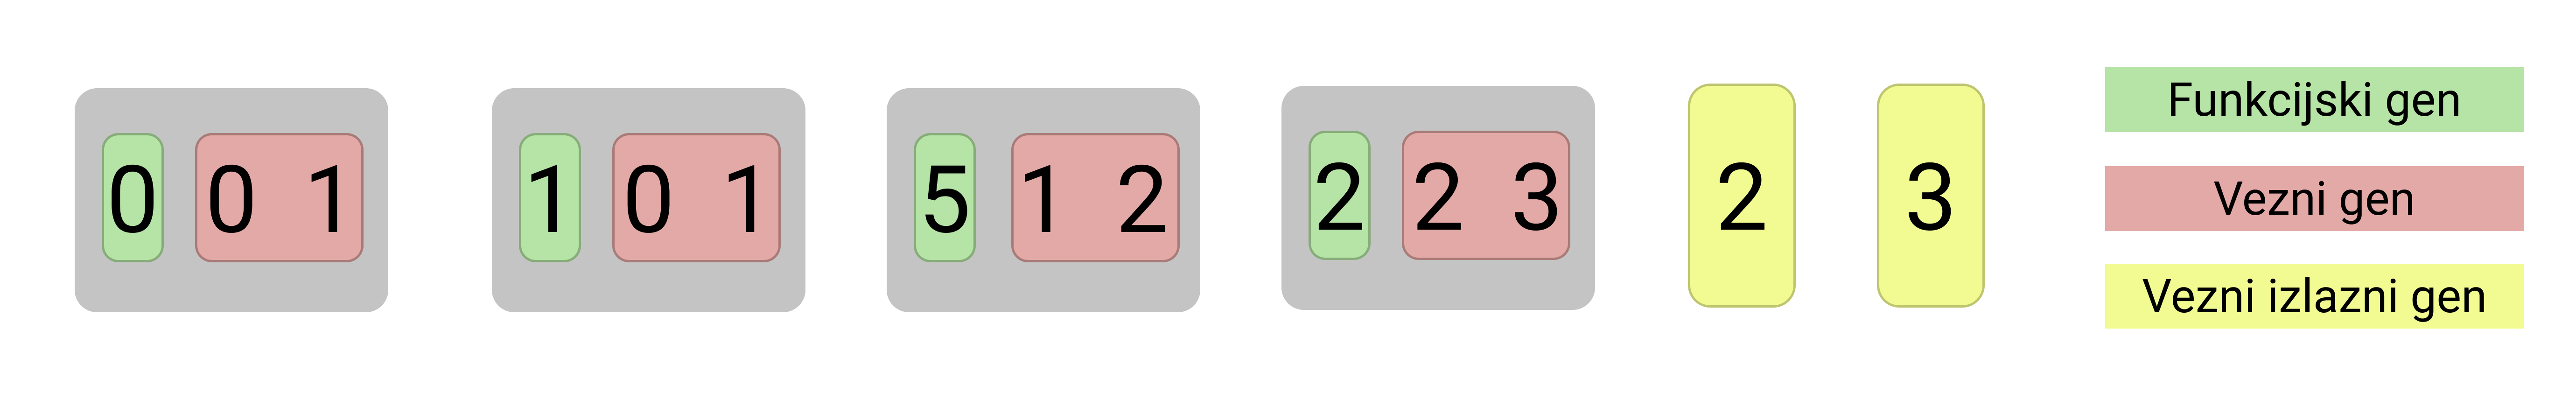
\includegraphics[width=\linewidth]{Illustrations/genotype.png}
	\caption{Primjer genotipa za CGP s dva ulaza, četiri sakrivena čvora i dva izlaza}
	\label{fig:genotype}
\end{figure}

\subsection{Arhitektura}
% Aciklički graf, dvodimenzionalnost, veličina, levelsback, nektivni čvor i kako utječe na fenotip
CGP jedinke prikazane su u obliku usmjerenih acikličnih grafova u dvodimenzionalnom prostoru (\cite{cgp}).
Arhitektura CGP jedinke definirana je sljedećim vrijednostima:
\begin{itemize}
	\item Broj ulaza $n_i$
	\item Broj izlaza $n_o$
	\item Broj skrivenih redaka i stupaca $n_r$ i $n_c$
	\item Broj najvećih vrijednost unazad koje čvor može uzimati (\emph{eng. levelsback}) $l$
\end{itemize}
Broj izlaza $>1$ nije tipična stvar za genetsko programiranje i veliki je benefit korištenja arhitekture inspirirane neuronskom mrežom.
Brojem najvećih vrijednosti unazad koje može čvor primiti definiramo složenost modela.
Priroda grafa je takva da se vrijednosti od prvog stupca šalju dublje sve do izlaza.
Ako je $l = 1$ definirali smo da svaki čvor može biti spojen najpliće u sloj prije sebe.
Tu mu dajemo manje slobode te ga ograničavamo na složenije modele nego da smo dozvolili $l > 1$.
Naravno, ako želimo dozvoliti spajanje s čvorom iz bilo kojeg stupca, postavljamo  $l=n_c$.

Parametrima $n_r$ i $n_c$ definiramo broj računalnih čvorova kao $L_n = n_r \times n_c$.
Imajući to na umu, ne moraju svi čvorovi biti iskorišteni.
Čvorove koji ne vode prema izlazu nazivamo ne-aktivnim (\emph{eng. non-coding}), njihovi ulazi i funkcija nemaju nikakav utjecaj na konačni izlaz iz mreže.
Tu je vidljiva razlika između genotipa koji ima fiksnu i konstantnu duljinu i fenotipa čija duljina i oblik ovise o aktivnim i neaktivnim čvorovima.
Na slici \ref{fig:cgp_gene_feno} vidljiv je genotip CGP mreže i pripadajući fenotip s jasno označenim ne-aktivnim čvorovima i pravilima indeksiranja.

\begin{figure}
	\centering
	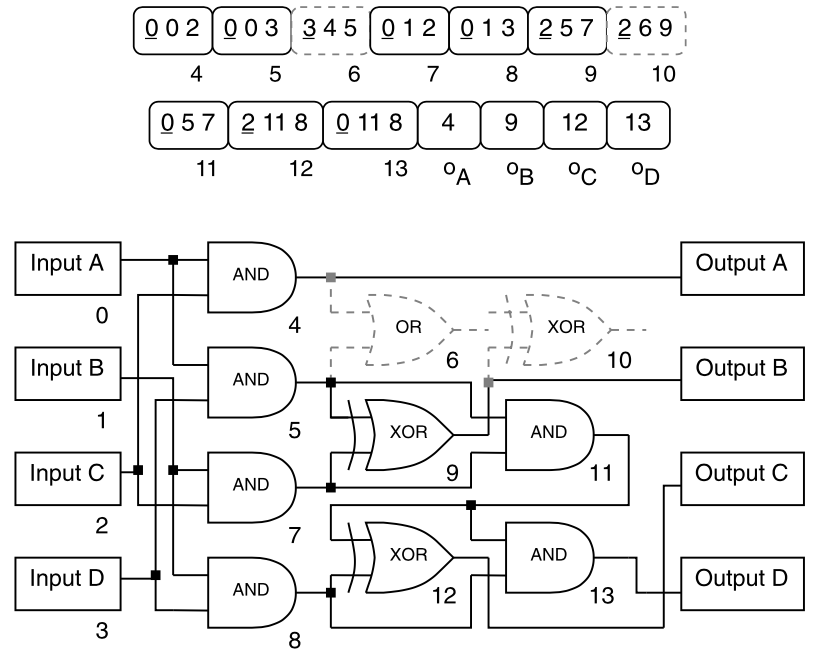
\includegraphics[width=\linewidth]{Illustrations/inactive_nodes.png}
	\caption{CGP genotip i fenotip digitalnog kruga. U čvorovima su vidljive funkcije koje izvode a čvorovi koji su iscrtani su neaktivni jer ne vode ni na jedan izlaz. Također su vidljivi indeksi svakog čvora i u genotipu i fenotipu. Izvor \cite{cgp}}
	\label{fig:cgp_gene_feno}
\end{figure}

I u praksi i u tablici \ref{table:function_table} vidljivo je da nemaju sve funkcije jednak broj ulaza.
Na primjer funkcija pod rednim brojem $4$, odnosno $\cos{x}$ ima jedan ulaz, dok funkcija $5$, $max(x, y)$ ima dva ulaza.
Treba li svakom čvoru dati točno onaj broj ulaza koliko traži njegova funkcija?
Naravno da ne, svako mutiranje mreže zahtjevalo bi ažuriranje broja ulaza u čvor i unjelo dodatnu kompleksnost u izvođenje te bi narušilo jednakost duljine genotipa svih jedinki.
Za svaku funkciju se zna njen broj ulaza (\emph{eng. arity}).
Ta vrijednost se iskoristi pri dodjeli broja ulaza čvorovima tako da svaki čvor dobije onoliko ulaza koliko prima funkcija s najvećim brojem ulaza.
Tako osiguravamo konstantnu duljinu genotipa i uklanjamo potrebu za ažuriranjem čvora pri promjeni funkcije iz npr. $cos{x}$ u $x + y$.

Prednost broja izlaza većeg od jedan vidljiva je na slici \ref{fig:cgp_gene_feno}.
Da se koristilo sintaksno stablo, bila bi potrebna četiri modela, jedan za svaki od izlaza A, B, C i D.
Velika prednost osjeti se i u obradi slike.
\cite{conv_gp} predstavio je obradu slike konvolucijskim metodama, inače rezerviranim za neuronske mreže, genetskim programiranjem.
Koristeći predložene metode, za pokušaje izlučivanja $n$ značajki (\emph{eng. feature}) potrebno je koristiti $n$ sintaksnih stabala.
U slučaju korištenja CGP-a, dovoljna je samo jedna jedinka za sve značajke.

\subsection{Evoluiranje}
